%package list
\documentclass{article}
\usepackage[top=3cm, bottom=3cm, outer=3cm, inner=3cm]{geometry}
\usepackage{multicol}
\usepackage{graphicx}
\usepackage{url}
%\usepackage{cite}
\usepackage{hyperref}
\usepackage{array}
%\usepackage{multicol}
\newcolumntype{x}[1]{>{\centering\arraybackslash\hspace{0pt}}p{#1}}
\usepackage{natbib}
\usepackage{pdfpages}
\usepackage{multirow}
\usepackage[normalem]{ulem}
\useunder{\uline}{\ul}{}
\usepackage{svg}
\usepackage{xcolor}
\usepackage{listings}
\lstdefinestyle{ascii-tree}{
    literate={├}{|}1 {─}{--}1 {└}{+}1 
  }
\lstset{basicstyle=\ttfamily,
  showstringspaces=false,
  commentstyle=\color{red},
  keywordstyle=\color{blue}
}
%\usepackage{booktabs}
\usepackage{caption}
\usepackage{subcaption}
\usepackage{float}
\usepackage{array}

\newcolumntype{M}[1]{>{\centering\arraybackslash}m{#1}}
\newcolumntype{N}{@{}m{0pt}@{}}


%%%%%%%%%%%%%%%%%%%%%%%%%%%%%%%%%%%%%%%%%%%%%%%%%%%%%%%%%%%%%%%%%%%%%%%%%%%%
%%%%%%%%%%%%%%%%%%%%%%%%%%%%%%%%%%%%%%%%%%%%%%%%%%%%%%%%%%%%%%%%%%%%%%%%%%%%
\newcommand{\itemEmail}{schirinosne@unsa.edu.pe}
\newcommand{\itemStudent}{Sebastian Arley Chirinos Negrón}
\newcommand{\itemCourse}{Estructura de datos y Algoritmos}
\newcommand{\itemCourseCode}{1702124}
\newcommand{\itemSemester}{I}
\newcommand{\itemUniversity}{Universidad Nacional de San Agustín de Arequipa}
\newcommand{\itemFaculty}{Facultad de Ingeniería de Producción y Servicios}
\newcommand{\itemDepartment}{Departamento Académico de Ingeniería de Sistemas e Informática}
\newcommand{\itemSchool}{Escuela Profesional de Ingeniería de Sistemas}
\newcommand{\itemAcademic}{2023 - A}
\newcommand{\itemInput}{Del 12 Junio2023}
\newcommand{\itemOutput}{Al 19 Junio 2023}
\newcommand{\itemPracticeNumber}{04}
\newcommand{\itemTheme}{Arbol Binario de Búsqueda}
%%%%%%%%%%%%%%%%%%%%%%%%%%%%%%%%%%%%%%%%%%%%%%%%%%%%%%%%%%%%%%%%%%%%%%%%%%%%
%%%%%%%%%%%%%%%%%%%%%%%%%%%%%%%%%%%%%%%%%%%%%%%%%%%%%%%%%%%%%%%%%%%%%%%%%%%%

\usepackage[english,spanish]{babel}
\usepackage[utf8]{inputenc}
\AtBeginDocument{\selectlanguage{spanish}}
\renewcommand{\figurename}{Figura}
\renewcommand{\refname}{Referencias}
\renewcommand{\tablename}{Tabla} %esto no funciona cuando se usa babel
\AtBeginDocument{%
	\renewcommand\tablename{Tabla}
}

\usepackage{fancyhdr}
\pagestyle{fancy}
\fancyhf{}
\setlength{\headheight}{30pt}
\renewcommand{\headrulewidth}{1pt}
\renewcommand{\footrulewidth}{1pt}
\fancyhead[L]{\raisebox{-0.2\height}{
\includegraphics[width=3cm]{img/logo_episunsa.png}}}
\fancyhead[C]{\fontsize{7}{7}\selectfont	\itemUniversity \\ \itemFaculty \\ \itemDepartment \\ \itemSchool \\ \textbf{\itemCourse}}
\fancyhead[R]{\raisebox{-0.2\height}{
\includegraphics[width=1.2cm]{img/logo_abet}}}
\fancyfoot[L]{Sebastian Chirinos Negrón}
\fancyfoot[C]{\itemCourse}
\fancyfoot[R]{Página \thepage}

% para el codigo fuente
\usepackage{listings}
\usepackage{color, colortbl}
\definecolor{dkgreen}{rgb}{0,0.6,0}
\definecolor{gray}{rgb}{0.5,0.5,0.5}
\definecolor{mauve}{rgb}{0.58,0,0.82}
\definecolor{codebackground}{rgb}{72, 0.95, 0.92}
\definecolor{tablebackground}{rgb}{0.8, 0, 0}

\lstset{frame=tb,
	language=bash,
	aboveskip=3mm,
	belowskip=3mm,
	showstringspaces=false,
	columns=flexible,
	basicstyle={\small\ttfamily},
	numbers=none,
	numberstyle=\tiny\color{gray},
	keywordstyle=\color{blue},
	commentstyle=\color{dkgreen},
	stringstyle=\color{mauve},
	breaklines=true,
	breakatwhitespace=true,
	tabsize=3,
	backgroundcolor= \color{codebackground},
}

\begin{document}
	
	\vspace*{10px}
	
	\begin{center}	
		\fontsize{17}{17} \textbf{ Informe de Laboratorio \itemPracticeNumber}
	\end{center}
	\centerline{\textbf{\Large Tema: \itemTheme}}
	%\vspace*{0.5cm}	

	\begin{flushright}
		\begin{tabular}{|M{2.5cm}|N|}
			\hline 
			\rowcolor{tablebackground}
			\color{white} \textbf{Nota}  \\
			\hline 
			     \\[30pt]
			\hline 			
		\end{tabular}
	\end{flushright}	

	\begin{table}[H]
		\begin{tabular}{|x{4.7cm}|x{4.8cm}|x{4.8cm}|}
			\hline 
			\rowcolor{tablebackground}
			\color{white} \textbf{Estudiante} & \color{white}\textbf{Escuela}  & \color{white}\textbf{Asignatura}   \\
			\hline 
			{\itemStudent \par \itemEmail} & \itemSchool & {\itemCourse \par Semestre: \itemSemester \par Código: \itemCourseCode}     \\
			\hline 			
		\end{tabular}
	\end{table}		
	
	\begin{table}[H]
		\begin{tabular}{|x{4.7cm}|x{4.8cm}|x{4.8cm}|}
			\hline 
			\rowcolor{tablebackground}
			\color{white}\textbf{Laboratorio} & \color{white}\textbf{Tema}  & \color{white}\textbf{Duración}   \\
			\hline 
			\itemPracticeNumber & \itemTheme & 04 horas   \\
			\hline 
		\end{tabular}
	\end{table}
	
	\begin{table}[H]
		\begin{tabular}{|x{4.7cm}|x{4.8cm}|x{4.8cm}|}
			\hline 
			\rowcolor{tablebackground}
			\color{white}\textbf{Semestre académico} & \color{white}\textbf{Fecha de inicio}  & \color{white}\textbf{Fecha de entrega}   \\
			\hline 
			\itemAcademic & \itemInput &  \itemOutput  \\
			\hline 
		\end{tabular}
	\end{table}
	
	\section{Tarea}
	\begin{itemize}
		\item Implementación de Árboles Binarios de Búsqueda:
		\item search(): Esta operación busca un elemento específico en el árbol binario de búsqueda. Comienza en la raíz y realiza comparaciones para determinar si el elemento buscado es menor, igual o mayor que el valor del nodo actual. Luego, se desplaza hacia el subárbol izquierdo o derecho según corresponda hasta encontrar el elemento o llegar a un nodo nulo.
		\item getMin(): Esta operación devuelve el valor mínimo almacenado en el árbol binario de búsqueda. Se realiza recorriendo siempre por los nodos más a la izquierda hasta llegar al nodo hoja más izquierdo.
		\item getMax(): Esta operación devuelve el valor máximo almacenado en el árbol binario de búsqueda. Se realiza recorriendo siempre por los nodos más a la derecha hasta llegar al nodo hoja más derecho.
		\item parent(): Esta operación devuelve el valor del nodo padre de un elemento dado en el árbol binario de búsqueda. Se realiza buscando el elemento y almacenando una referencia al nodo padre durante el recorrido.
		\item son(): Esta operación verifica si un elemento dado tiene hijos en el árbol binario de búsqueda. Se realiza buscando el elemento y verificando si tiene nodos hijos izquierdo o derecho.
		\item insert(): Esta operación permite insertar un nuevo elemento en el árbol binario de búsqueda. Comienza comparando el nuevo elemento con el valor del nodo actual y se desplaza hacia el subárbol izquierdo o derecho según corresponda hasta encontrar una posición vacía para la inserción.
		\item remove(): Esta operación permite eliminar un elemento específico del árbol binario de búsqueda. Se realiza buscando el elemento y aplicando diferentes casos dependiendo de si el nodo a eliminar es una hoja, tiene un solo hijo o tiene dos hijos.
		\item INPUT: Una sola palabra en mayúsculas.
		\item OUTPUT: Se debe construir el árbol binario de búsqueda considerando el valor decimal de su código ASCII.
		\item Pruebas de las operaciones implementadas: Para verificar el correcto funcionamiento de las operaciones, se realizarán pruebas utilizando diferentes palabras y se mostrarán los resultados obtenidos.
		\item Estudio de la librería Graph Stream: Se investigará la librería Graph Stream para obtener una salida gráfica de la implementación del árbol binario de búsqueda. Se explorarán las funcionalidades y se evaluará su viabilidad para representar visualmente la estructura y los nodos del árbol.
		\item Se aplicarán todas las recomendaciones dadas por el docente para asegurar una implementación eficiente y correcta del árbol binario de búsqueda.
	\end{itemize}
		

	\section{URL de Repositorio Github}
	\begin{itemize}
		\item URL del Repositorio GitHub para clonar o recuperar.
		\item \url{https://github.com/BastleyNait/EDA-LAB-B-23A.git}
		\item URL para el laboratorio 04 en el Repositorio GitHub.
		\item \url{https://github.com/BastleyNait/EDA-LAB-B-23A/tree/main/lab03}
	\end{itemize}
	
	\section{Ejercicios designados}

	\subsection{Clase Bst}
	\begin{itemize}	
		\item  
		Un BST (Binary Search Tree, por sus siglas en inglés) es una estructura de datos jerárquica utilizada para almacenar elementos de manera ordenada y permitir búsquedas eficientes. Consiste en un árbol binario en el que cada nodo tiene un valor asociado y dos hijos, uno izquierdo y otro derecho. La propiedad principal de un BST es que el valor de cada nodo en el subárbol izquierdo es menor que el valor del nodo y el valor de cada nodo en el subárbol derecho es mayor. Esto facilita la búsqueda de un elemento específico en el árbol, ya que se puede comparar el valor buscado con los valores de los nodos y seguir el camino apropiado hacia la izquierda o la derecha según corresponda. Además de las operaciones de búsqueda, los BST también admiten inserción, eliminación y recorridos en orden, preorden y postorden.
	\end{itemize}	
	
	\lstinputlisting[language=Java, caption={Bst.java},numbers=left,]{src/Bst.java}	

	\begin{itemize}
		\item \textbf{Line 1:} Importa la clase ExceptionNoFound del paquete myExceptions.
		\item \textbf{Line 3:} Declaración de la clase Bst que utiliza un tipo genérico T que extiende la interfaz Comparable.
		\item \textbf{Line 4:} Declaración del atributo root de tipo Nodo<T>, que representa la raíz del árbol binario de búsqueda.
		\item \textbf{Line 6-9:} Constructor de la clase Bst que inicializa el atributo root como nulo.
		\item \textbf{Line 11-14:} Método getter para obtener el valor del atributo root.
		\item \textbf{Line 16-19:} Método setter para establecer el valor del atributo root.
		\item \textbf{Line 21-24:} Método que verifica si el árbol binario de búsqueda está vacío. Retorna true si el atributo root es nulo.
		\item \textbf{Line 26-36:} Método insert() que permite insertar un nuevo elemento en el árbol binario de búsqueda. Recibe el elemento a insertar y el nodo actual. Compara el elemento con el valor del nodo actual y se desplaza hacia el subárbol izquierdo o derecho según corresponda hasta encontrar una posición vacía para la inserción. Si el elemento ya existe en el árbol, lanza una excepción de tipo ExceptionNoFound.
		\item \textbf{Line 38-61:} Método search() que busca un elemento específico en el árbol binario de búsqueda. Recibe el elemento a buscar y el nodo actual. Realiza comparaciones para determinar si el elemento buscado es menor, igual o mayor que el valor del nodo actual y se desplaza hacia el subárbol izquierdo o derecho según corresponda. Retorna el nodo encontrado. Si el elemento no se encuentra en el árbol, lanza una excepción de tipo ExceptionNoFound.
		\item \textbf{Line 63-76:} Método getMin() que devuelve el valor mínimo almacenado en el árbol binario de búsqueda. Recibe un nodo y se desplaza siempre por los nodos más a la izquierda hasta llegar al nodo hoja más izquierdo. Retorna el valor mínimo encontrado. Si el árbol está vacío, lanza una excepción de tipo ExceptionNoFound.
		\item \textbf{Line 78-91:} Método getMax() que devuelve el valor máximo almacenado en el árbol binario de búsqueda. Recibe un nodo y se desplaza siempre por los nodos más a la derecha hasta llegar al nodo hoja más derecho. Retorna el valor máximo encontrado. Si el árbol está vacío, lanza una excepción de tipo ExceptionNoFound.
		\item \textbf{Line 93-102:} Método parent() que devuelve el valor del nodo padre de un elemento dado en el árbol binario de búsqueda. Recibe el elemento a buscar y el nodo actual. Busca el nodo padre durante el recorrido y retorna su valor. Si el nodo no tiene padre, lanza una excepción de tipo ExceptionNoFound.
		\item \textbf{Line 104-139:} Método remove() que permite eliminar un elemento específico del árbol

	%%%%%%%%%%%%%%%%%%%%%%%%%%%%%%%%%%%%%%%%%%%%%%%%%%%%%%%%%%%%%%%%%%%%%%%%%%%%%%%%%%%%%%%%%%%%%
	\subsection{Clase Nodo}
	\begin{itemize}	
		\item  El código proporcionado define la clase Nodo que se utiliza en la implementación de un árbol binario de búsqueda. Los nodos contienen un valor y referencias a los nodos hijos izquierdo y derecho. También se incluyen métodos getter y setter para acceder y modificar los atributos del nodo, así como un método toString() para representar el valor del nodo como una cadena.

	\end{itemize}	
	
	\lstinputlisting[language=Java, caption={Nodo.java},numbers=left,]{src/Nodo.java}	

	\begin{itemize}
		\item \textbf{Line 1:} Declaración de la clase Nodo con un parámetro de tipo genérico T.
		\item \textbf{Line 3:} Declaración del atributo data de tipo T, que almacena el valor del nodo.
		\item \textbf{Line 5-7:} Declaración de los atributos left y right de tipo Nodo<T>, que representan los hijos izquierdo y derecho del nodo respectivamente.
		\item \textbf{Line 9-11:} Constructor de la clase Nodo que recibe el valor del nodo, el nodo hijo izquierdo y el nodo hijo derecho. Inicializa los atributos correspondientes con los valores proporcionados.
		\item \textbf{Line 13-16:} Constructor sobrecargado de la clase Nodo que recibe solo el valor del nodo. Llama al constructor principal con los valores proporcionados y establece los hijos izquierdo y derecho como nulos.
		\item \textbf{Line 18-21:} Método getter para obtener el valor del atributo data.
		\item \textbf{Line 23-26:} Método setter para establecer el valor del atributo data.
		\item \textbf{Line 28-31:} Método getter para obtener el nodo hijo izquierdo.
		\item \textbf{Line 33-36:} Método setter para establecer el nodo hijo izquierdo.
		\item \textbf{Line 38-41:} Método getter para obtener el nodo hijo derecho.
		\item \textbf{Line 43-46:} Método setter para establecer el nodo hijo derecho.
		\item \textbf{Line 48-51:} Método toString() que devuelve una representación en cadena del valor del nodo.
	\end{itemize}
%%%%%%%%%%%%%%%%%%%%%%%%%%%%%%%%%%%%%%%%%%%%%%%%%%%%%%%%%%%%%%%%%%%%%%%%%%%%%%%%%%%%%%%%%%%%%%%%%%%%%%%%%%
%%%%%%%%%%%%%%%%%%%%%%%%%%%%%%%%%%%%%%%%%%%%%%%%%%%%%%%%%%%%%%%%%%%%%%%%%%%%%%%%%%%%%%%%%%%%%
\subsection{Clase Aplication}
\begin{itemize}	
	\item  El código proporcionado define la clase Nodo que se utiliza en la implementación de un árbol binario de búsqueda. Los nodos contienen un valor y referencias a los nodos hijos izquierdo y derecho. También se incluyen métodos getter y setter para acceder y modificar los atributos del nodo, así como un método toString() para representar el valor del nodo como una cadena.

\end{itemize}	
\lstinputlisting[language=Java, caption={Aplication.java},numbers=left,]{src/Aplicacion.java}	
\begin{itemize}
	\item \textbf{Line 10:} Método principal main que se ejecuta al iniciar la aplicación. Llama al método generar().
	\item \textbf{Line 13-15:} Método generar() que genera el árbol binario de búsqueda, crea y muestra el grafo utilizando la biblioteca GraphStream, y realiza diversas operaciones en el árbol.
	\item \textbf{Line 17:} Establece la propiedad del sistema "org.graphstream.ui" a "swing". Esta propiedad configura el renderizador de GraphStream para utilizar la interfaz de usuario de Swing.
	\item \textbf{Line 19-20:} Crea un objeto Graph llamado graph utilizando la implementación SingleGraph. Este objeto representa el grafo que se visualizará.
	\item \textbf{Line 22-23:} Crea un objeto Viewer y lo asocia al grafo graph. El Viewer se utiliza para visualizar el grafo en una ventana.
	\item \textbf{Line 24:} Deshabilita el diseño automático del grafo. Esto evita que los nodos se reorganicen automáticamente.
	\item \textbf{Line 26-27:} Establece una hoja de estilo para el grafo. Define cómo se mostrarán los nodos y las aristas en la visualización.
	\item \textbf{Line 28-30:} Crea un objeto Scanner para leer la entrada del usuario.
	\item \textbf{Line 31-33:} Solicita al usuario que ingrese una palabra en mayúsculas y la guarda en la variable word.
	\item \textbf{Line 35-37:} Crea un objeto Bst<String> llamado bst utilizando la implementación de un árbol binario de búsqueda. Este árbol se utilizará para almacenar los caracteres de la palabra.
	\item \textbf{Line 38:} Inicializa la variable i con el valor 0.
	\item \textbf{Line 40-42:} Convierte la palabra en un arreglo de caracteres.
	\item \textbf{Line 43-66:} Itera sobre cada carácter en el arreglo de caracteres.
	\item \textbf{Line 45-61:} Dentro del bucle, se realiza lo siguiente:
	\begin{itemize}
	\item Se intenta buscar el carácter en el árbol utilizando el método search(). Si la búsqueda es exitosa, se lanza una excepción ExceptionNoFound, que indica que el elemento ya existe en el árbol.
	\item Si no se produce una excepción, se inserta el carácter junto con un sufijo numérico en el árbol utilizando el método insert().
	\item Si se produce una excepción ExceptionNoFound, se captura y se imprime la traza de la excepción.
	\end{itemize}
	\item \textbf{Line 68-69:} Agrega los nodos y aristas al grafo graph utilizando el método addNodesToGraph(). El método recorre el árbol y agrega los nodos correspondientes al grafo, así como las aristas que los conectan.
	\item \textbf{Line 70-71:} Crea un nuevo objeto Graph llamado graph2 utilizando la implementación SingleGraph. Este objeto representa el segundo grafo en el que se mostrará el árbol después de realizar la eliminación de un nodo.
	\item \textbf{Line 73:} Establece la hoja de estilo para el grafo graph2 de manera similar a como se hizo para el grafo graph.
	\item \textbf{Line 74-76:} Crea un objeto Viewer asociado al grafo graph2, que se utilizará para visualizar el grafo en una ventana.
	\item \textbf{Line 77:} Deshabilita el diseño automático del grafo graph2.
	\item \textbf{Line 79-80:} Solicita al usuario que ingrese una letra a eliminar y la guarda en la variable eliminar.
	\item \textbf{Line 81-82:} Llama al método remove(eliminar) del árbol binario de búsqueda bst para eliminar el nodo correspondiente a la letra ingresada.
	\item \textbf{Line 83:} Remueve el nodo correspondiente a la letra ingresada del grafo graph.
	\item \textbf{Line 84-85:} Agrega los nodos y aristas actualizados al grafo graph2 utilizando nuevamente el método addNodesToGraph().
	\item \textbf{Line 87-88:} Imprime el mínimo valor del árbol binario de búsqueda utilizando el método getMin().
	\item \textbf{Line 89-90:} Crea un nuevo nodo en el grafo graph2 representando el mínimo valor del árbol y lo posiciona en la visualización.
	\item \textbf{Line 92-93:} Imprime el máximo valor del árbol binario de búsqueda utilizando el método getMax().
	\item \textbf{Line 94-95:} Crea un nuevo nodo en el grafo graph2 representando el máximo valor del árbol y lo posiciona en la visualización.
	\item \textbf{Line 97-98:} Solicita al usuario que ingrese una letra a buscar y la guarda en la variable buscar.
	\item \textbf{Line 99-100:} Realiza una búsqueda en el árbol binario de búsqueda utilizando el método search(buscar).
	\item \textbf{Line 101-102:} Realiza una búsqueda del padre de la letra ingresada utilizando el método parent(buscar).
	\item \textbf{Line 103-104:} Crea un nuevo nodo en el grafo graph2 representando el resultado de la búsqueda y lo posiciona en la visualización.
	\item \textbf{Line 105-106:} Crea un nuevo nodo en el grafo graph2 representando el resultado de la búsqueda del padre y lo posiciona en la visualización.
	\item \textbf{Line 108-109:} Solicita al usuario que ingrese una letra para buscar sus hijos y la guarda en la variable son.
	\end{itemize}

%%%%%%%%%%%%%%%%%%%%%%%%%%%%%%%%%%%%%%%%%%%%%%%%%%%%%%%%%%%%%%%%%%%%%%%%%%%%%%%%%%%%%%%%%%%%%%%%%%

\begin{itemize}	
	\item Ejecucion del codigo:
\end{itemize}	

\begin{figure}[H]
	\centering
	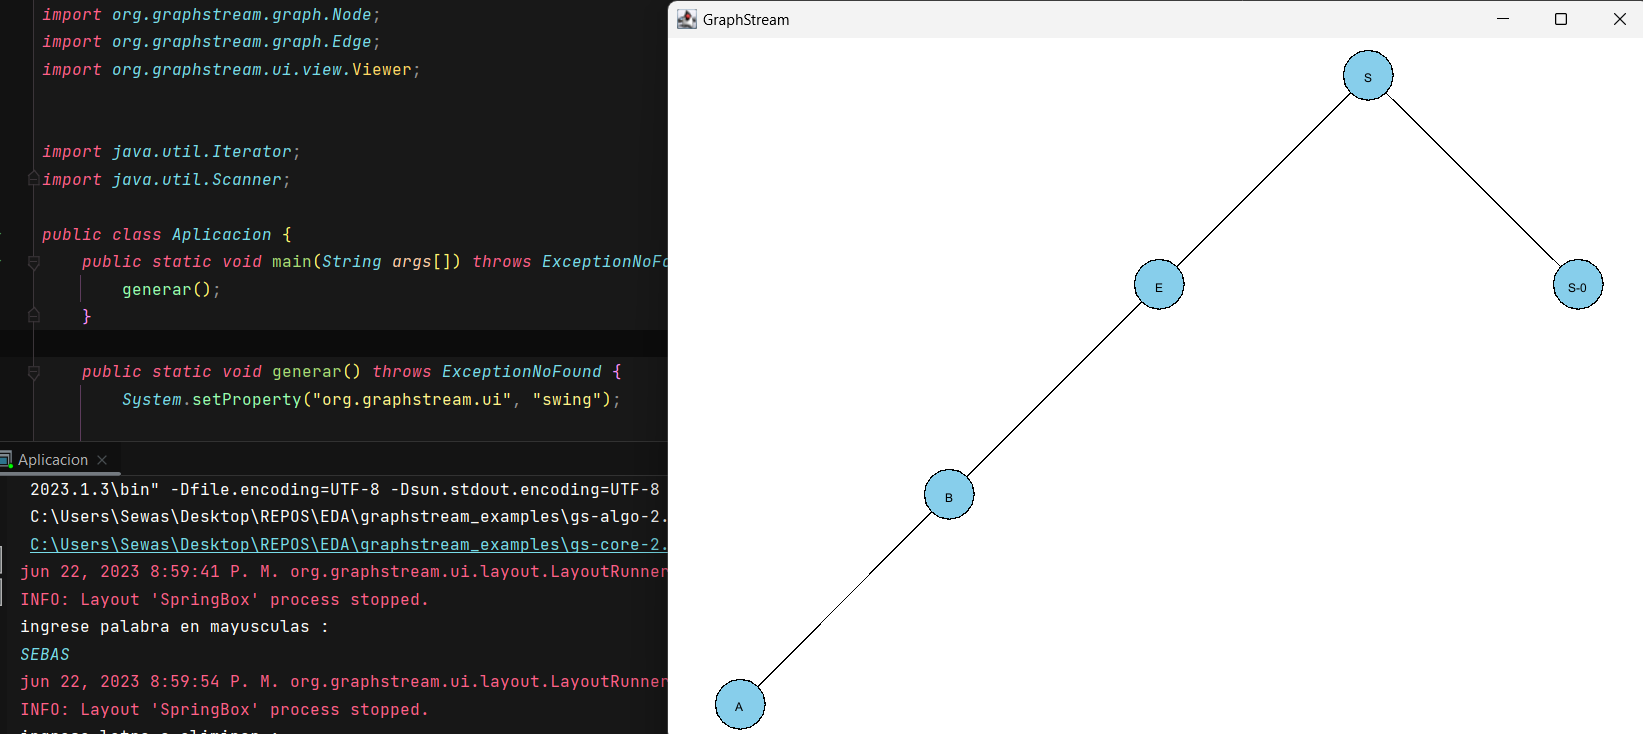
\includegraphics[width=0.7\textwidth,keepaspectratio]{img/ejecucion1.png}
	%\includesvg{img/automata.svg}
	%\label{img:mot2}
	%\caption{Product backlog.}
\end{figure}

\begin{figure}[H]
	\centering
	\includegraphics[width=0.7\textwidth,keepaspectratio]{img/ejecucion2.png}
	%\includesvg{img/automata.svg}
	%\label{img:mot2}
	%\caption{Product backlog.}
\end{figure}

%%%%%%%%%%%%%%%%%%%%%%%%%%%%%%%%%%%%%%%%%%%%%%%%%%%%%%%%%%%%%%%%%%%%%%%%%%%%%%%%%%


	\subsection{Commits del trabajo}
	\begin{itemize}	
		\item Acá estan algunos de los commits mas importantes en este trabajo:
	\end{itemize}	
	
	\begin{figure}[H]
		\centering
		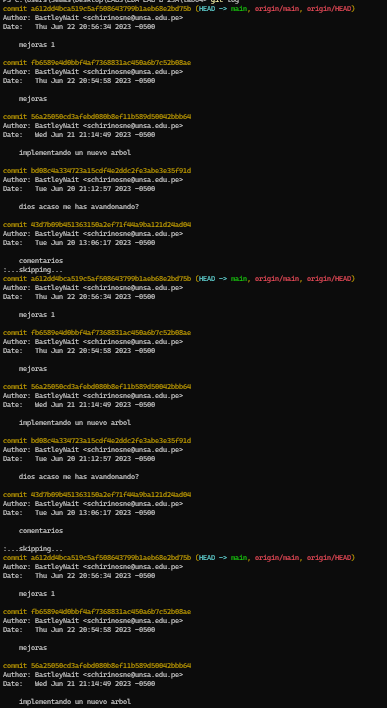
\includegraphics[width=0.7\textwidth,keepaspectratio]{img/Commits.png}
		%\includesvg{img/automata.svg}
		%\label{img:mot2}
		%\caption{Product backlog.}
	\end{figure}


%%%%%%%%%%%%%%%%%%%%%%%%%%%%%%%%%%%%%%%%%%%%%%%%%%%%%%%%%%%%%%%%%%%%%%%%%%%%%%%%%%
	
		
	\subsection{Estructura de laboratorio 04}
	\begin{itemize}	
		\item El contenido que se entrega en este laboratorio es el siguiente:
	\end{itemize}
	
\begin{lstlisting}[style=ascii-tree]
lab04/
|   .gitignore
|   Bst.java
|   Nodo.java
|   Aplication.java

\---latex
    |	EDA_lab04_schirinosne.pdf
    |   EDA_lab04_schirinosne.tex
    |
    +---img
    |       Commits.png
    |       ejecucion1.png
	|       ejecucion2.png
    |       logo_abet.png
    |       logo_episunsa.png
    |       logo_unsa.jpg
    |
    \---src
	|		Bst.java
	|		Nodo.java
	|		Aplication.java
	|		
	\---myExceptions
			ExceptionIsEmpty.java
			ExceptionNoFound.java
               
\end{lstlisting}    

\section{¿Explique como es el algoritmo que implement ́o para obtener el  ́arbol binario de b ́usqueda con
la libreria Graph Stream? Recuerde que pueden haber operaciones sobre el BST.
}
\begin{itemize}
	\item Se utiliza la biblioteca GraphStream para visualizar el árbol binario de búsqueda.
	\item Se crea un objeto Graph utilizando la implementación SingleGraph para representar el grafo.
	\item Se crea un objeto Viewer y se asocia al grafo para visualizarlo en una ventana.
	\item Se deshabilita el diseño automático del grafo para evitar reorganizaciones automáticas de los nodos.
	\item Se establece una hoja de estilo para definir la apariencia de los nodos y las aristas en la visualización.
	\item Se lee una palabra en mayúsculas ingresada por el usuario.
	\item Se crea un árbol binario de búsqueda y se insertan los caracteres de la palabra en el árbol.
	\item Se agregan los nodos y las aristas correspondientes al grafo para representar el árbol.
	\item Se muestra el grafo que representa el árbol binario de búsqueda.
\end{itemize}		
	\section{\textcolor{red}{Rúbricas}}
	
	\subsection{\textcolor{red}{Entregable Informe}}
	\begin{table}[H]
		\caption{Tipo de Informe}
		\setlength{\tabcolsep}{0.5em} % for the horizontal padding
		{\renewcommand{\arraystretch}{1.5}% for the vertical padding
		
		\begin{tabular}{|p{3cm}|p{12cm}|}
			\hline
			\multicolumn{2}{|c|}{\textbf{\textcolor{red}{Informe}}}  \\
			\hline 
			\textbf{\textcolor{red}{Latex}} & \textcolor{blue}{El informe está en formato PDF desde Latex,  con un formato limpio (buena presentación) y facil de leer.}   \\ 
			\hline 
			
			
		\end{tabular}
	}
	\end{table}
	\subsection{\textcolor{red}{Rúbrica para el contenido del Informe y demostración}}
	\begin{itemize}			
		\item El alumno debe marcar o dejar en blanco en celdas de la columna \textbf{Checklist} si cumplio con el ítem correspondiente.
		\item Si un alumno supera la fecha de entrega,  su calificación será sobre la nota mínima aprobada, siempre y cuando cumpla con todos lo items.
		\item El alumno debe autocalificarse en la columna \textbf{Estudiante} de acuerdo a la siguiente tabla:
	
		\begin{table}[ht]
			\caption{Niveles de desempeño}
			\begin{center}
			\begin{tabular}{ccccc}
    			\hline
    			 & \multicolumn{4}{c}{Nivel}\\
    			\cline{1-5}
    			\textbf{Puntos} & Insatisfactorio 25\%& En Proceso 50\% & Satisfactorio 75\% & Sobresaliente 100\%\\
    			\textbf{2.0}&0.5&1.0&1.5&2.0\\
    			\textbf{4.0}&1.0&2.0&3.0&4.0\\
    		\hline
			\end{tabular}
		\end{center}
	\end{table}	
	
	\end{itemize}
	
	\begin{table}[H]
		\caption{Rúbrica para contenido del Informe y demostración}
		\setlength{\tabcolsep}{0.5em} % for the horizontal padding
		{\renewcommand{\arraystretch}{1.5}% for the vertical padding
		%\begin{center}
		\begin{tabular}{|p{2.7cm}|p{7cm}|x{1.3cm}|p{1.2cm}|p{1.5cm}|p{1.1cm}|}
			\hline
    		\multicolumn{2}{|c|}{Contenido y demostración} & Puntos & Checklist & Estudiante & Profesor\\
			\hline
			\textbf{1. GitHub} & Hay enlace URL activo del directorio para el  laboratorio hacia su repositorio GitHub con código fuente terminado y fácil de revisar. &2 &X &2 & \\ 
			\hline
			\textbf{2. Commits} &  Hay capturas de pantalla de los commits más importantes con sus explicaciones detalladas. (El profesor puede preguntar para refrendar calificación). &4 & x&4 & \\ 
			\hline 
			\textbf{3. Código fuente} &  Hay porciones de código fuente importantes con numeración y explicaciones detalladas de sus funciones. &2 &X &2 & \\ 
			\hline 
			\textbf{4. Ejecución} & Se incluyen ejecuciones/pruebas del código fuente  explicadas gradualmente. &2 &X &2 & \\ 
			\hline			
			\textbf{5. Pregunta} & Se responde con completitud a la pregunta formulada en la tarea.  (El profesor puede preguntar para refrendar calificación).  &2 &X &2 & \\ 
			\hline	
			\textbf{6. Fechas} & Las fechas de modificación del código fuente estan dentro de los plazos de fecha de entrega establecidos. &2 &X &0 & \\ 
			\hline 
			\textbf{7. Ortografía} & El documento no muestra errores ortográficos. &2 &X &2 & \\ 
			\hline 
			\textbf{8. Madurez} & El Informe muestra de manera general una evolución de la madurez del código fuente,  explicaciones puntuales pero precisas y un acabado impecable.   (El profesor puede preguntar para refrendar calificación).  &4 &x &4 & \\ 
			\hline
			\multicolumn{2}{|c|}{\textbf{Total}} &20 & &18 & \\ 
			\hline
		\end{tabular}
		%\end{center}
		%\label{tab:multicol}
		}
	\end{table}
	
\clearpage		
\section{Referencias}
\begin{itemize}			
	\item \url{https://algorithmtutor.com/Data-Structures/Tree/Binary-Trees/}
	\item \url{https://algorithmtutor.com/Data-Structures/Tree/Binary-Search-Trees/}
	\item \url{https://github.com/rescobedoq/graphstream_examples}

\end{itemize}	

	
%\clearpage
%\bibliographystyle{apalike}
%\bibliographystyle{IEEEtranN}
%\bibliography{bibliography}
			
\end{document}